Оптимальное распределение ресурсов в аналитических постановках изучается с помощью дизайна механизмов.
Современный подход был предложен и развит Леонидом Гурвичем \cite{hurwicz1960optimality}.
В его работе изучается проблемы доказательная эффективность организации рабочих процессов.

Механизм позволяет ограничить свободу действий игроков в системе таким образом, 
что действия агентов в доминантных стратегиях будут соответствовать ожиданиям принципала.

Строгое определение вводится через понятие байесовых игр с неполной информацией, 
предполагающих наличие нескольких многошаговых игр, направленных на формирование оптимальной стратегии. 


\begin{figure}[h]
    \centering
    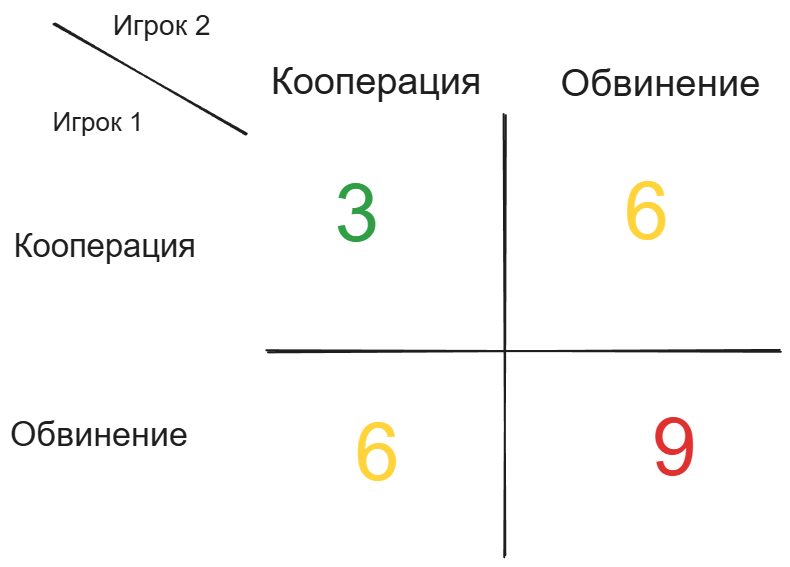
\includegraphics[width=0.5\textwidth]{assets/pedagogic/social/dilemma.excalidraw.png}
    \caption{Дилемма заключенного}
    \label{dilemma}
\end{figure}


\textit{Определение} \textbf{Байесова игра} это набор исходов $(N,O,\Theta)$ таких что,
\begin{itemize}
    \item $\mathbf{N}$ конечное множество агентов $n$
    \item $O$ множество исходов
    \item  $\Theta = \Theta_1 \times \Theta_2 \dots \Theta_n $ множество 
    \item $u = (u_1, \dots, u_N)$, где $u_i: O \times \Theta \rightarrow \mathrm{R}$  функция полезности для игрока $i$
\end{itemize}

\textit{Определение} \textbf{Механизм} для байесовой игры это пара $(A,M)$, где \begin{itemize}
    \item $A = A_1 \times \dots \times A_n$ набор действий доступный агенту $i$
    \item $M: A \rightarrow \Pi(O)$ соединяет действия с распределением возможностей
\end{itemize}


Изучение механизма заключается в анализе доминантных стратегий и равновесных состояний, к которым они приводят. 

\textit{Определение} В заданной байесовой игре, механизм является \textbf{воплощением доминантной стартегии} 
социального выбора функции $C$, если для любого вектора полезности $u$ , 
у игры есть равновесие в доминантной стратегии, и для любого равновесия $a^*$ выполняется $M(a^*) = C(u)$


Теория механизмов используется В постановках с ассиметричной информацией
и достаточно большим числом игроков, чтокак правило не позволяет наивно перебрать возможные исходы.

\begin{figure}[h]
    \centering
    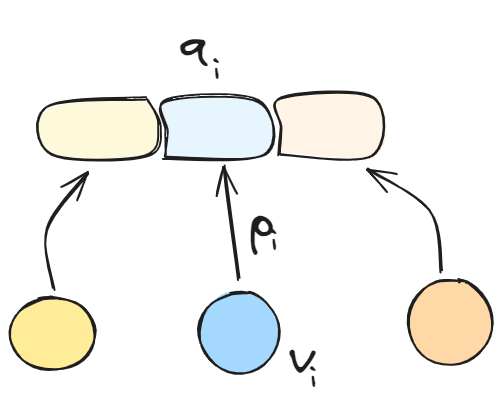
\includegraphics[width=0.5\textwidth]{assets/pedagogic/social/mech.excalidraw.png}
    \caption{Механизм определяет распределение ресурса $\mathbf{x}$ и платежа $\mathbf{p}$ в зависимости от ставок $\mathbf{b}$}
    \label{utility}
\end{figure}

Каждый игрок $i$ имеетx четверка $(v_i,b_i,p_i)$, соответствующую \begin{itemize}
    \item случайную величину $v_i$ с функцией распределения $F$. Обозначим полученный квантиль распределения $q(v_i) = 1 - F(v_i)$.
    \item ставка на лот $b_i$.
    \item доля полученного ресурса $x_i$
    \item $p_i$ итоговый платеж
\end{itemize}

Тогда функция полезности для каждого игрока $i$ при заданном векторе ставок запишется как 
\begin{equation}
    u_i(\mathbf{b};q_i) = v(q_i) \cdot x_i(\mathbf{b})   
\end{equation}

\textit{} Байес-Нэшевым равновесием называют результат распределения, в котором каждый участник аукциона
максимизирует свою функцию утилитарности $u_i$ как матожидание от квантилей $q_{-i}$.

\begin{equation}
    \max_{\mathbf{q},\mathbf{b}} \mathrm{E}_{\mathbf{q_{-i}}}\left[u_i(\mathbf{b}(\mathbf{q});q_i)\right] \left[\right] 
\end{equation}

\begin{figure}[h]
    \centering
    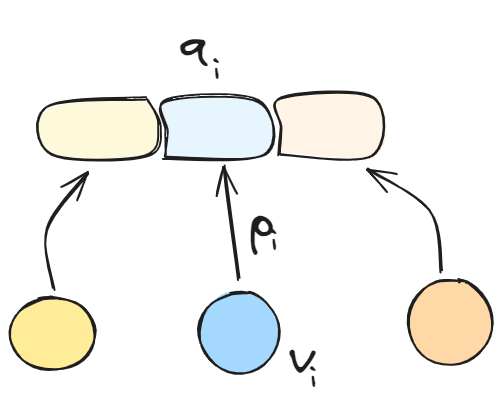
\includegraphics[width=0.5\textwidth]{assets/pedagogic/social/mech.excalidraw.png}
    \caption{Ресурсное распределение}
    \label{utility}
\end{figure}


В теории \cite{bulow1989simple} аукционов различают платеж . Формально опишем условия: \begin{itemize}
    \item $\tilde{x}_i(\mathbf{q}) = x_i(\mathbf{b}(\mathbf{q}))$ фактическое (от \textit{англ.} ex-post) полученная доля ресурса;
    \item $\hat{x}_i(q_i) = \mathrm{E}_\mathbf{q} \left[\tilde{x_i(\mathbf{q}),q_i}\right]$ текущее(от \textit{англ.} interim) ресурсное ожидание;
    \item $\hat{p}$ ожидаемый платеж.
\end{itemize}


\textit{Лемма} Набор имеет Байес-Нэшево равновесие при условии \begin{itemize}
    \item $\hat{x_i}(q_i)$ монотонно убывает по $q_i$
    \item $\hat{p}_i(q_i) = v(q_i) \cdot \hat{x}_i(q_i) + \int_{q_i}^1 \hat{x}_i \cdot v'(z) dz$
\end{itemize}
Заданные условия достаточны для достижения уникально равновесия $\mathbf{b}$. Доказательство приведено в \cite{myerson1981optimal}.


Одним из примером механизма являются рейтинг системы, широко распространенные в спортивных интеллектуальных соревнованиях.

\textit{Рейтинг-система} – это модель, которая ранжирует
участников  в единый линейный порядок поданным сравнений небольших подмножеств этих игроков.
 
В этом случае рейтинг можно задать как оператор $\zeta$ принимающий на вход потенциалы, задающие силу объекта.
\begin{equation}
    p(x_i \succ x_j) = \zeta(\phi(x_i),\phi(x_j))
\end{equation}
Согласно модели рейтинга Эло сила игрока задается случайной величиной $\xi$. 
Экспоненциальный вид графика связан с предположением о том, что в стратегических играх существенное различие в навыке гарантирует победу
\textit{Рейтинг} задается матожиданием силы $\mathcal{E} \xi$.
Согласно модели Эло сила игрока задается нормально, причем дисперсия $\sigma$ фиксирована для всех игроков
Тогда сила игры согласно предположению определяется как:
\begin{equation}
    p(x) = \frac{1}{\sigma \sqrt{2\pi}} \exp^{- \frac{1}{2\sigma^2}{(x-s)^2}}
\end{equation}
Таким образом, рейтинг является латентной переменной. В литературе также популярна модель Брэдли-Терри,задающая
вероятность победы зависит как:
\begin{equation}
    P(\theta)
\end{equation}
Заметим, что подмена $\gamma ~ exp(-\theta/\beta^2)$ позволяет отождествить подходы.
В шахматной практике волатильность считается определенной и имеет стандартное отклонение равное 20:
\begin{equation}
    \frac{1}{1+10^\frac{R_B-R_A}{400}} 
\end{equation}













